\documentclass[11pt,a4paper]{article}

\usepackage[utf8]{inputenc}
\usepackage{graphicx}
\usepackage{amsmath}
\usepackage[colorlinks=true, linkcolor=blue, urlcolor=blue, citecolor=blue]{hyperref}
\usepackage{geometry}
\usepackage{booktabs}
\usepackage{float}
\usepackage{subcaption}
\usepackage{listings}
\usepackage{xcolor}
\usepackage{array}
\usepackage{tabularx}
\usepackage{parskip}
\usepackage{titlesec}
\usepackage{fancyhdr}
\usepackage{setspace}

\geometry{top=1in, bottom=1in, left=1.2in, right=1.2in}
\setstretch{1.15}

% Header and footer
\pagestyle{fancy}
\fancyhf{}
\rhead{COM 763 Advanced Machine Learning}
\lhead{Portfolio Task 1}
\cfoot{\thepage}
\renewcommand{\headrulewidth}{0.4pt}

% Section formatting
\titleformat{\section}{\large\bfseries}{\thesection.}{1em}{}[\titlerule]
\titleformat{\subsection}{\normalsize\bfseries}{\thesubsection}{1em}{}

% Code listing style
\lstset{
  language=Python,
  backgroundcolor=\color{gray!10},
  basicstyle=\ttfamily\footnotesize,
  keywordstyle=\color{blue}\bfseries,
  commentstyle=\color{green!60!black},
  stringstyle=\color{orange!80!black},
  numbers=left,
  numberstyle=\tiny\color{gray},
  stepnumber=1,
  numbersep=5pt,
  frame=single,
  breaklines=true,
  captionpos=b,
  tabsize=4
}

% ----------------------------------------------------------------
\title{%
  \vspace{-1cm}
  \textbf{COM 763 Advanced Machine Learning}\\[0.5em]
  \large Portfolio Task 1: Wine Quality Prediction System\\[0.3em]
  \normalsize A Complete Machine Learning Development Report
}
\author{Student ID: [Your ID] \\ Wrexham University}
\date{\today}
% ----------------------------------------------------------------

\begin{document}

\maketitle
\thispagestyle{empty}

% ---------------------------------------------------------------
\begin{abstract}
\noindent
This report documents the design, development, evaluation, and deployment of a complete machine learning system that predicts wine quality from physicochemical measurements. The project addresses a real-world quality control problem in the wine industry, where subjective human tasting is expensive and inconsistent at scale. A \textbf{binary classification} approach is adopted, distinguishing between ``Good'' (quality score $\geq$ 6) and ``Bad'' (quality score $<$ 6) wines. Two models were trained and compared: \textbf{Logistic Regression} and a \textbf{Random Forest Classifier} tuned via \texttt{GridSearchCV}. The Random Forest achieved superior performance and was selected as the final model. The system was deployed as an interactive web application on Streamlit Community Cloud.

\smallskip
\noindent\textbf{Streamlit Application URL:} \url{https://proect-wine.streamlit.app}

\smallskip
\noindent\textbf{GitHub Repository:} \url{https://github.com/[your-username]/Proect-Wine}
\end{abstract}

\tableofcontents
\newpage

% ================================================================
\section{Problem Definition and System Framing}
% ================================================================

\subsection{The Real-World Problem}

The global wine industry is a multi-billion-dollar market in which product quality is a primary driver of consumer purchasing decisions and brand reputation. Traditionally, wine quality is assessed by a panel of expert human tasters (sommeliers) who assign a quality score based on sensory attributes such as aroma, taste, and finish. This approach, while effective for premium releases, suffers from several significant limitations when applied at industrial scale:

\begin{itemize}
    \item \textbf{Subjectivity:} Quality scores can vary widely between different tasters, introducing inconsistency.
    \item \textbf{Cost and Time:} Maintaining a qualified tasting panel is expensive and slow; wines must be assessed bottle by bottle.
    \item \textbf{Scalability:} As production volumes increase, the bottleneck created by manual assessment becomes increasingly problematic.
    \item \textbf{Feedback Latency:} Tasting panels evaluate the final product, making it difficult to correct production issues early in the process.
\end{itemize}

During the wine production process, chemical analysis is already routinely performed to measure physicochemical properties such as acidity, sugar content, alcohol level, and sulphate concentration. These measurements are objective, cheap to obtain, and available at multiple stages of production. The central question this project addresses is: \textit{Can these objective chemical measurements be used to reliably predict whether a wine will be rated as ``Good'' quality by a human taster?}

\subsection{Justification for Machine Learning}

This problem is well-suited to machine learning for the following reasons:

\begin{enumerate}
    \item \textbf{Complex, Non-Linear Relationships:} Wine quality is not determined by a single feature in isolation. For example, it is not simply the case that ``higher alcohol always means better wine.'' The interaction between alcohol, acidity, sulphates, and other features determines quality in a complex, non-linear way that is difficult to model with simple rules.

    \item \textbf{Large Historical Data Availability:} The existence of labelled datasets (where historical chemical measurements are paired with expert quality scores) provides the supervised learning signal needed to train a predictive model.

    \item \textbf{Consistency:} Once trained, a machine learning model applies the same decision boundary every time, eliminating the inter-rater variability inherent in human assessment.

    \item \textbf{Integration with Existing Processes:} Since chemical testing is already part of the production workflow, an ML model can be integrated to provide quality predictions automatically, with no additional data collection overhead.
\end{enumerate}

\subsection{Task Framing}

The machine learning task is formally defined as a \textbf{supervised binary classification} problem:

\begin{itemize}
    \item \textbf{Inputs (Features):} Eleven continuous, objective physicochemical measurements: \textit{fixed acidity, volatile acidity, citric acid, residual sugar, chlorides, free sulfur dioxide, total sulfur dioxide, density, pH, sulphates,} and \textit{alcohol}.

    \item \textbf{Target Variable:} A binary label derived from the original 10-point quality score. Quality scores of 6, 7, or 8 are mapped to \textbf{1 (Good)}; scores of 3, 4, or 5 are mapped to \textbf{0 (Bad)}. This framing reflects the practical business decision of whether a wine meets the standard for a commercial release.

    \item \textbf{Success Criteria:} The model should achieve a high F1-score (balancing precision and recall) and a high ROC-AUC score, since both false positives (mislabelling bad wine as good) and false negatives (rejecting acceptable wine) carry business costs.
\end{itemize}

\begin{figure}[H]
    \centering
    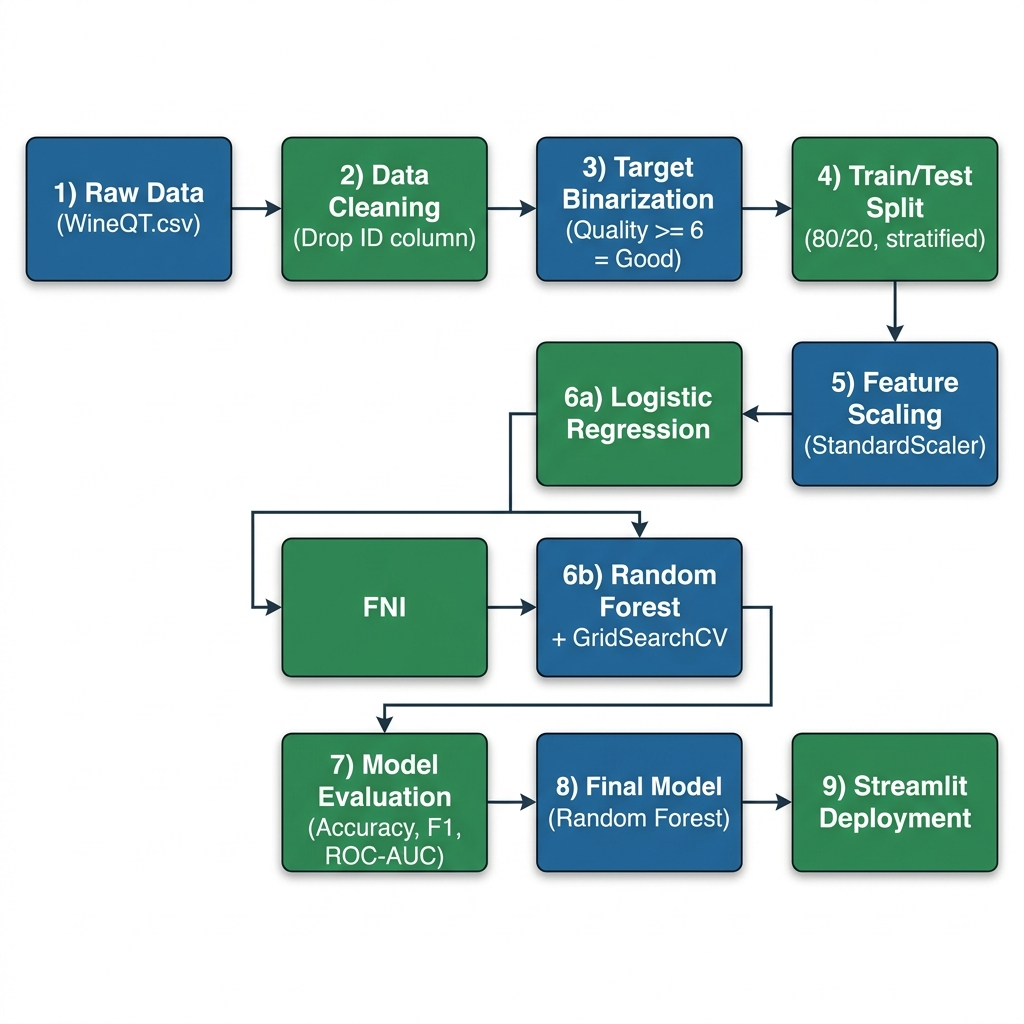
\includegraphics[width=\textwidth]{figures/pipeline_diagram.png}
    \caption{End-to-end machine learning pipeline for the Wine Quality Prediction System.}
    \label{fig:pipeline}
\end{figure}

% ================================================================
\section{Data Pipeline and Feature Handling}
% ================================================================

\subsection{Dataset Overview}

The dataset used in this project is the \textbf{Wine Quality Dataset} (\texttt{WineQT.csv}), a well-established benchmark dataset for classification tasks. Key characteristics are summarised in Table~\ref{tab:dataset}.

\begin{table}[H]
    \centering
    \caption{Dataset Summary}
    \label{tab:dataset}
    \begin{tabular}{ll}
        \toprule
        \textbf{Property} & \textbf{Detail} \\
        \midrule
        Number of samples & 1,143 \\
        Number of raw columns & 13 \\
        Number of features (after cleaning) & 11 \\
        Quality score range & 3 to 8 \\
        Missing values & None \\
        Target class (Good, score $\geq$ 6) & 618 samples \\
        Target class (Bad, score $<$ 6) & 525 samples \\
        \bottomrule
    \end{tabular}
\end{table}

The eleven physicochemical features and their real-world meaning are described in Table~\ref{tab:features}.

\begin{table}[H]
    \centering
    \caption{Description of Physicochemical Features}
    \label{tab:features}
    \begin{tabularx}{\textwidth}{lX}
        \toprule
        \textbf{Feature} & \textbf{Description} \\
        \midrule
        Fixed Acidity & Most acids involved with wine (tartaric acid), which are not volatile (do not evaporate readily). \\
        Volatile Acidity & Amount of acetic acid, which at high levels can lead to an unpleasant vinegar taste. \\
        Citric Acid & Found in small quantities, can add freshness and flavour. \\
        Residual Sugar & Amount of sugar remaining after fermentation stops; affects sweetness. \\
        Chlorides & Amount of salt in the wine. \\
        Free Sulfur Dioxide & Prevents microbial growth and wine oxidation. \\
        Total Sulfur Dioxide & Total amount of SO\textsubscript{2} in free and bound forms. \\
        Density & Density of the wine, closely related to alcohol and sugar content. \\
        pH & Acidity or basicity of the wine on a scale of 0--14. \\
        Sulphates & A wine additive that contributes to SO\textsubscript{2} levels. \\
        Alcohol & Percentage of alcohol content. \\
        \bottomrule
    \end{tabularx}
\end{table}

\subsection{Exploratory Data Analysis}

An initial inspection of the dataset confirmed \textbf{no missing values} in any column, which simplified the cleaning process. Figure~\ref{fig:quality_dist} shows the distribution of the original quality scores, revealing that the dataset is concentrated around scores of 5 and 6, with very few examples at the extremes (3 and 8). This imbalance at the extremes is an important observation, as it means the model will have fewer examples to learn from at the boundary of the ``Good''/``Bad'' threshold.

\begin{figure}[H]
    \centering
    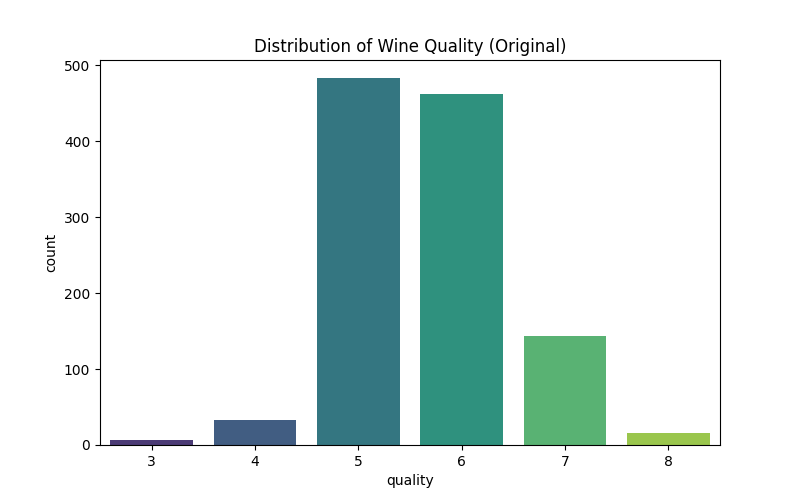
\includegraphics[width=0.75\textwidth]{figures/quality_distribution.png}
    \caption{Distribution of the original wine quality scores (3--8). The dataset is heavily concentrated around scores 5 and 6.}
    \label{fig:quality_dist}
\end{figure}

The correlation heatmap (Figure~\ref{fig:heatmap}) reveals the linear relationships between all variables. Key observations include:

\begin{itemize}
    \item \textbf{Alcohol} has the strongest positive correlation with quality (0.48), suggesting that wines with higher alcohol content tend to be rated higher.
    \item \textbf{Volatile Acidity} has a notable negative correlation with quality (--0.41), confirming that a sour, vinegar-like taste detracts from perceived quality.
    \item \textbf{Fixed Acidity} and \textbf{Density} are strongly correlated (0.68), and similarly \textbf{Fixed Acidity} and \textbf{Citric Acid} (0.67), indicating some multicollinearity among features.
    \item \textbf{Free Sulfur Dioxide} and \textbf{Total Sulfur Dioxide} are highly correlated (0.66), as expected, since free SO\textsubscript{2} is a component of total SO\textsubscript{2}.
\end{itemize}

\begin{figure}[H]
    \centering
    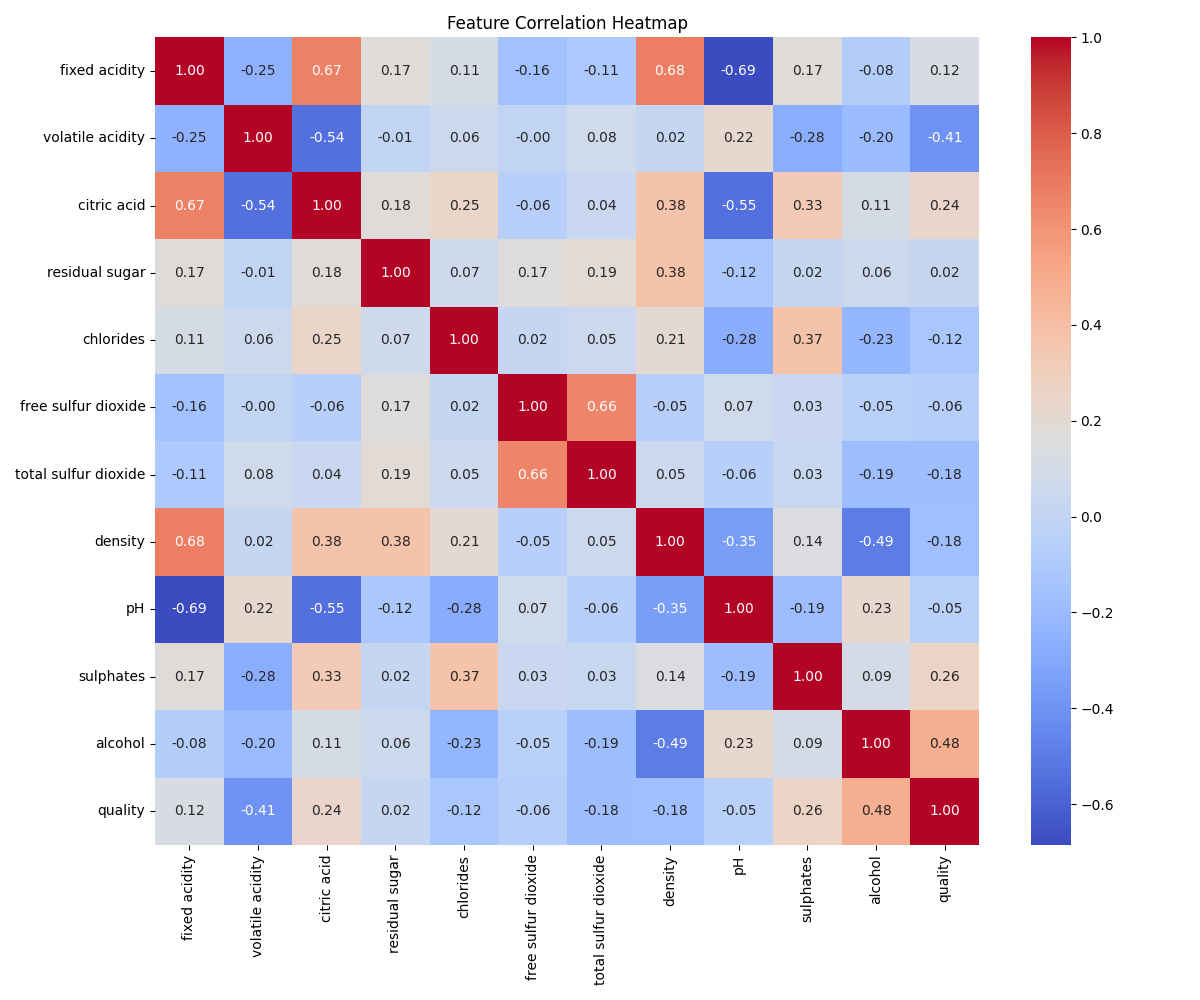
\includegraphics[width=\textwidth]{figures/correlation_heatmap.png}
    \caption{Correlation heatmap of all features and the quality target. Colour intensity indicates correlation strength (red = positive, blue = negative).}
    \label{fig:heatmap}
\end{figure}

\subsection{Data Cleaning}

The following cleaning steps were applied:

\begin{enumerate}
    \item \textbf{Removal of the `Id' Column:} The dataset contains an arbitrary integer `Id' column that serves only as a row identifier. It carries no predictive information and was removed to prevent the model from learning spurious correlations with this index.

    \item \textbf{Target Binarization:} The original quality score (a 6-class integer from 3 to 8) was transformed into a binary label. A threshold of 6 was chosen based on the conventional wine industry interpretation where a score of 6 or above is considered commercially acceptable. This resulted in 618 ``Good'' wines and 525 ``Bad'' wines (Figure~\ref{fig:binary_dist}), giving a reasonably balanced class distribution suitable for standard classification.
\end{enumerate}

\begin{figure}[H]
    \centering
    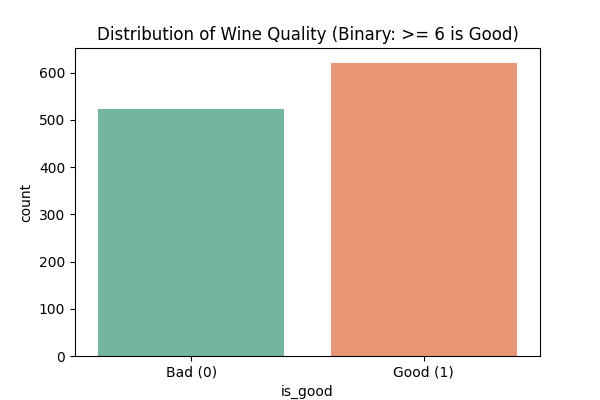
\includegraphics[width=0.6\textwidth]{figures/binary_distribution.png}
    \caption{Distribution of the binarized target variable. ``Good'' (score $\geq$ 6): 618 samples; ``Bad'' (score $<$ 6): 525 samples.}
    \label{fig:binary_dist}
\end{figure}

\subsection{Feature Engineering and Scaling}

After cleaning, the dataset was split into features $X$ (11 columns) and the target $y$ (\texttt{is\_good}). A stratified 80/20 train-test split was applied (\texttt{random\_state=42}) to ensure the class distribution was preserved in both sets.

The physicochemical features operate on vastly different numerical scales. For example, \texttt{total sulfur dioxide} values can exceed 100, while \texttt{chlorides} values are typically below 0.1. This scale disparity presents a significant challenge for distance-based and gradient-based algorithms:

\begin{itemize}
    \item In \textbf{Logistic Regression}, gradient descent operates in the feature space. When features are on different scales, the loss function's contours become elongated ellipses, causing gradient descent to oscillate and converge very slowly, or not at all within a limited number of iterations.
    \item In \textbf{Random Forest}, scaling is less critical since the algorithm uses decision boundaries based on feature thresholds, not distances. However, scaling was applied uniformly for consistency and to facilitate a fair comparison.
\end{itemize}

\textbf{Solution:} All 11 features were standardized using Scikit-learn's \texttt{StandardScaler}, which transforms each feature to have a mean of 0 and a standard deviation of 1. Critically, the scaler was \texttt{fit} only on the \textbf{training data} and then \texttt{transform} was applied to both the training and test sets. This prevents \textit{data leakage}, where information from the test set could inadvertently influence the preprocessing step.

\begin{figure}[H]
    \centering
    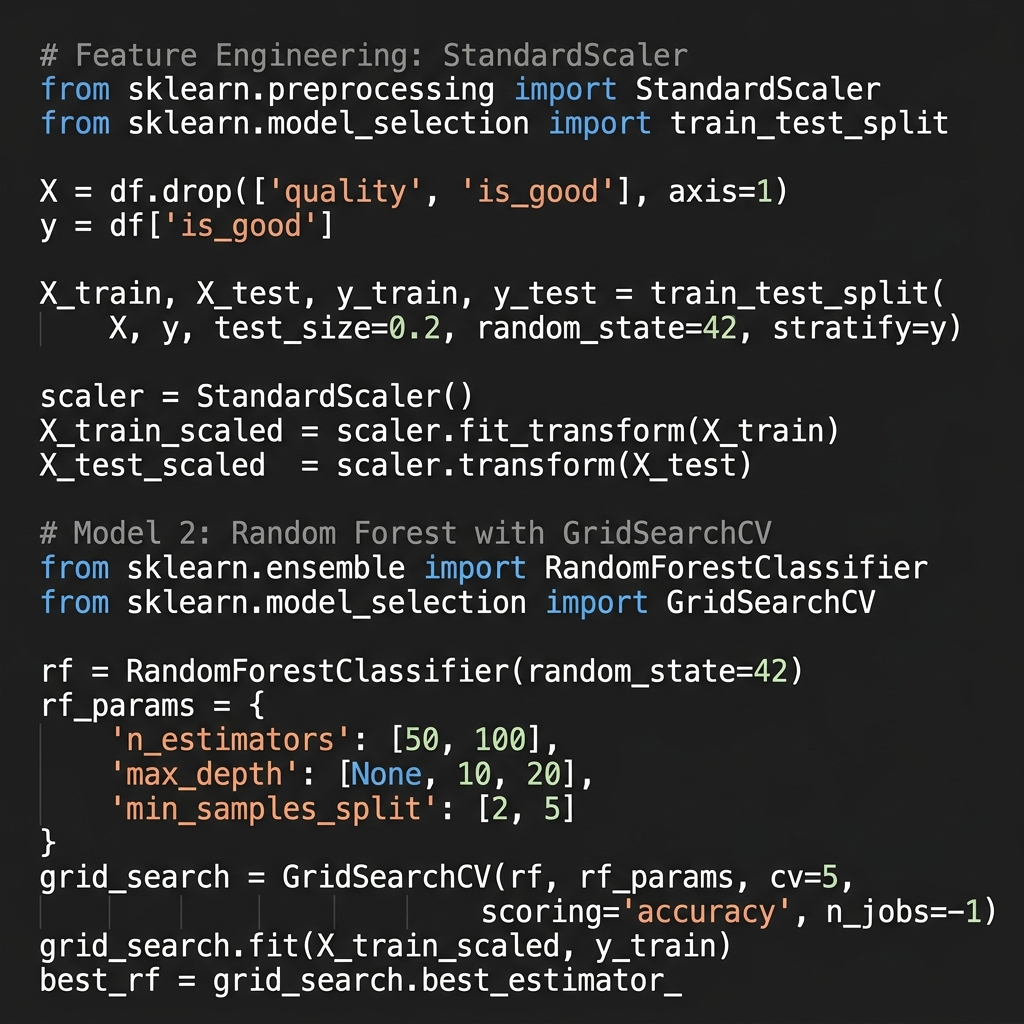
\includegraphics[width=0.9\textwidth]{figures/code_screenshot.png}
    \caption{Key code section showing the train-test split, StandardScaler application, and Random Forest GridSearchCV implementation.}
    \label{fig:code}
\end{figure}

% ================================================================
\section{Model Implementation and Debugging}
% ================================================================

\subsection{Model Selection Rationale}

Two candidate models were chosen to represent different ends of the complexity spectrum:

\textbf{Model 1: Logistic Regression}

Logistic Regression was chosen as the \textit{baseline linear model}. Despite its simplicity, it offers several advantages in this context:
\begin{itemize}
    \item \textbf{Interpretability:} The learned coefficients directly indicate the direction and magnitude of each feature's influence on the predicted quality.
    \item \textbf{Speed:} It trains very quickly, making it ideal for rapid prototyping and comparison.
    \item \textbf{Calibration:} The probability outputs from Logistic Regression are well-calibrated, which is useful for interpreting the confidence of predictions.
\end{itemize}

\textbf{Model 2: Random Forest Classifier}

A Random Forest was chosen as the \textit{non-linear ensemble model}. Its advantages include:
\begin{itemize}
    \item \textbf{Handles Non-linearity:} Wine quality is likely determined by complex, non-linear interactions between chemical properties that a linear model cannot capture.
    \item \textbf{Robustness to Overfitting:} By averaging predictions from many decision trees (each trained on a random subset of data and features), the ensemble is far more robust to overfitting than a single decision tree.
    \item \textbf{Feature Importance:} Random Forests provide a built-in measure of feature importance, offering valuable insight into which chemical properties most influence quality.
    \item \textbf{No Scaling Requirement:} Unlike Logistic Regression, Random Forests are not sensitive to feature scale.
\end{itemize}

\subsection{Implementation Details}

\textbf{Logistic Regression} was initialised with \texttt{random\_state=42} and trained on the scaled training data (\texttt{X\_train\_scaled}).

\textbf{Random Forest} was initialised with \texttt{random\_state=42} and tuned using \texttt{GridSearchCV} with 5-fold cross-validation. The hyperparameter search space was:

\begin{table}[H]
    \centering
    \caption{Hyperparameter Grid for Random Forest Tuning}
    \label{tab:gridsearch}
    \begin{tabular}{lll}
        \toprule
        \textbf{Hyperparameter} & \textbf{Values Searched} & \textbf{Best Value} \\
        \midrule
        \texttt{n\_estimators} & 50, 100 & 100 \\
        \texttt{max\_depth} & None, 10, 20 & None (fully grown) \\
        \texttt{min\_samples\_split} & 2, 5 & 2 \\
        \bottomrule
    \end{tabular}
\end{table}

The scoring metric for \texttt{GridSearchCV} was \texttt{accuracy}, and the search evaluated 12 hyperparameter combinations across 5 folds ($12 \times 5 = 60$ model fits in total). The best estimator identified was a Random Forest with 100 trees, unconstrained depth, and a minimum of 2 samples required to split an internal node.

\subsection{Debugging Narrative: Convergence Warning in Logistic Regression}

During the initial development phase, a significant issue was encountered with the Logistic Regression model. The model was initially trained on the \textit{raw, unscaled} data as a first quick test.

\textbf{The Problem:} The training run immediately produced a \texttt{ConvergenceWarning}:

\begin{lstlisting}[language=bash, caption=ConvergenceWarning observed during initial training on unscaled data]
ConvergenceWarning: lbfgs failed to converge (status=1):
STOP: TOTAL NO. of ITERATIONS REACHED LIMIT.
Increase the number of iterations (max_iter) or scale the data
as shown in:
  https://scikit-learn.org/stable/modules/preprocessing.html
\end{lstlisting}

Furthermore, the accuracy and F1-score of this initial run were noticeably lower than expected, suggesting the model had not found an optimal decision boundary.

\textbf{Root Cause Analysis:} The issue was caused by the disparity in feature scales. When \texttt{total sulfur dioxide} (values up to 289) and \texttt{chlorides} (values around 0.01--0.6) are in the same feature space, the gradient of the loss function is dominated by the large-magnitude feature. The gradient descent algorithm (L-BFGS solver) struggles to navigate this poorly-scaled loss landscape efficiently, requiring many more iterations than the default \texttt{max\_iter=100} to converge.

\textbf{The Fix:} The solution was to apply \texttt{StandardScaler} to the data before training. After standardization, all features had approximately equal influence on the gradient magnitude, and the L-BFGS solver converged without warnings in far fewer iterations. The improvement in classification metrics after applying the fix was clear evidence that scaling had resolved the issue.

\textbf{Key Learning:} This debugging experience reinforced the critical importance of feature preprocessing for gradient-based models. It is good practice to always scale data before applying Logistic Regression, Support Vector Machines, or any neural network.

% ================================================================
\section{Experimental Evaluation and Model Selection}
% ================================================================

\subsection{Evaluation Methodology}

Both models were evaluated on the 20\% hold-out test set (229 samples) that was not seen during training or hyperparameter tuning. The following evaluation metrics were used:

\begin{itemize}
    \item \textbf{Accuracy:} The proportion of all predictions (both Good and Bad) that were correct. While intuitive, accuracy can be misleading with imbalanced classes.
    \item \textbf{Precision:} Of all wines predicted as ``Good'', what proportion were actually good? High precision means few false alarms.
    \item \textbf{Recall:} Of all wines that were truly ``Good'', what proportion did the model correctly identify? High recall means the model misses few good wines.
    \item \textbf{F1-Score:} The harmonic mean of Precision and Recall. This is the primary metric for comparing models, as it balances both concerns.
    \item \textbf{ROC-AUC:} The Area Under the Receiver Operating Characteristic Curve measures the model's overall discriminative ability, independent of any specific classification threshold. A score of 1.0 indicates a perfect classifier; 0.5 indicates a random guesser.
\end{itemize}

\subsection{Quantitative Results}

The performance metrics for both models on the test set are summarised in Table~\ref{tab:results}.

\begin{table}[H]
    \centering
    \caption{Test Set Performance Metrics: Logistic Regression vs. Random Forest}
    \label{tab:results}
    \begin{tabular}{lcccc}
        \toprule
        \textbf{Model} & \textbf{Accuracy} & \textbf{Precision} & \textbf{Recall} & \textbf{F1-Score} \\
        \midrule
        Logistic Regression & 0.7729 & 0.8017 & 0.7824 & 0.7919 \\
        Random Forest       & \textbf{0.8079} & \textbf{0.8090} & \textbf{0.8550} & \textbf{0.8314} \\
        \bottomrule
    \end{tabular}
\end{table}

The Random Forest outperformed Logistic Regression on every metric. Most notably, its Recall of 0.855 (compared to 0.782 for Logistic Regression) indicates that it is significantly better at correctly identifying wines that are truly ``Good'', which is the primary business objective.

\subsection{Confusion Matrix Analysis}

The confusion matrices in Figure~\ref{fig:cm} provide a detailed breakdown of prediction outcomes.

\begin{figure}[H]
    \centering
    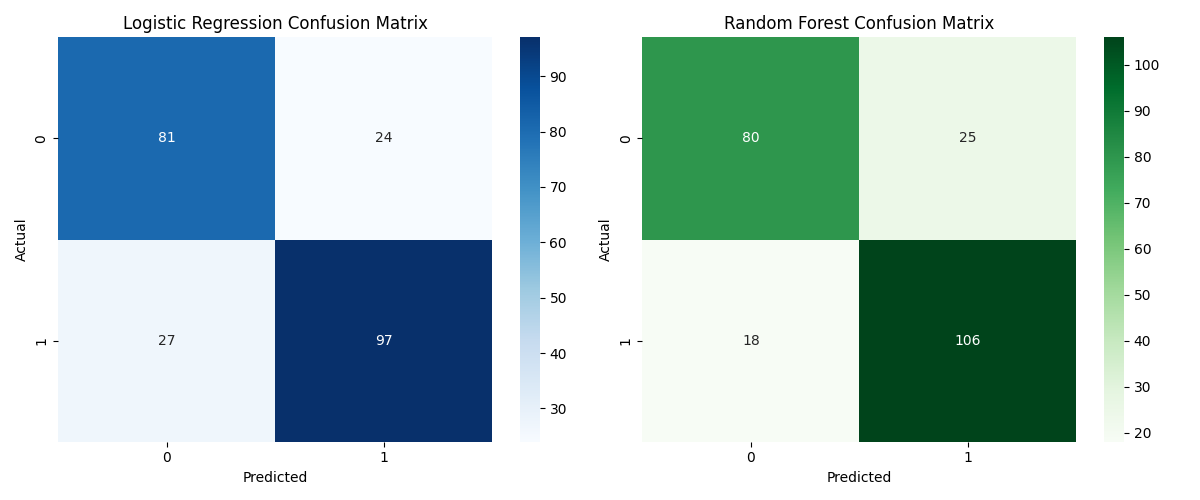
\includegraphics[width=\textwidth]{figures/confusion_matrices.png}
    \caption{Confusion matrices for Logistic Regression (left) and Random Forest (right) on the test set. Rows represent actual labels; columns represent predicted labels.}
    \label{fig:cm}
\end{figure}

Reading the confusion matrices (class 0 = Bad, class 1 = Good):

\begin{itemize}
    \item \textbf{Logistic Regression:} 81 True Negatives (correct ``Bad'' predictions), 24 False Positives (``Bad'' wines incorrectly labelled ``Good''), 27 False Negatives (``Good'' wines incorrectly labelled ``Bad''), and 97 True Positives.

    \item \textbf{Random Forest:} 80 True Negatives, 25 False Positives, 18 False Negatives, and 106 True Positives. The Random Forest achieved 9 fewer False Negatives, meaning it correctly identified 9 additional good wines that the Logistic Regression missed. For a wine producer, this represents less good product being incorrectly rejected.
\end{itemize}

\subsection{ROC Curve Analysis}

The ROC curves (Figure~\ref{fig:roc}) plot the True Positive Rate against the False Positive Rate at every possible classification threshold.

\begin{figure}[H]
    \centering
    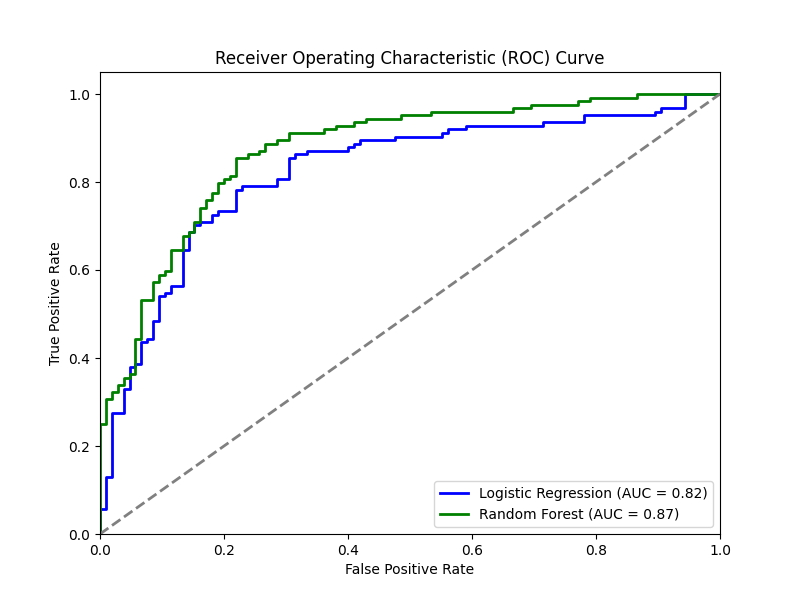
\includegraphics[width=0.8\textwidth]{figures/roc_curves.png}
    \caption{ROC curves comparing Logistic Regression (AUC = 0.82) and Random Forest (AUC = 0.87). The closer the curve is to the top-left corner, the better the model's discriminative ability.}
    \label{fig:roc}
\end{figure}

The Random Forest achieves an AUC of \textbf{0.87} compared to the Logistic Regression's AUC of \textbf{0.82}. This 5-point AUC advantage confirms that the Random Forest has significantly stronger overall discriminative power across all classification thresholds. This is particularly meaningful in practice, as it allows the decision threshold to be adjusted to suit different business priorities without a major degradation in overall performance.

\subsection{Feature Importance Analysis}

One of the key advantages of the Random Forest is its ability to provide feature importance scores (Figure~\ref{fig:feat_imp}). These scores represent the mean decrease in node impurity (Gini importance) attributable to each feature.

\begin{figure}[H]
    \centering
    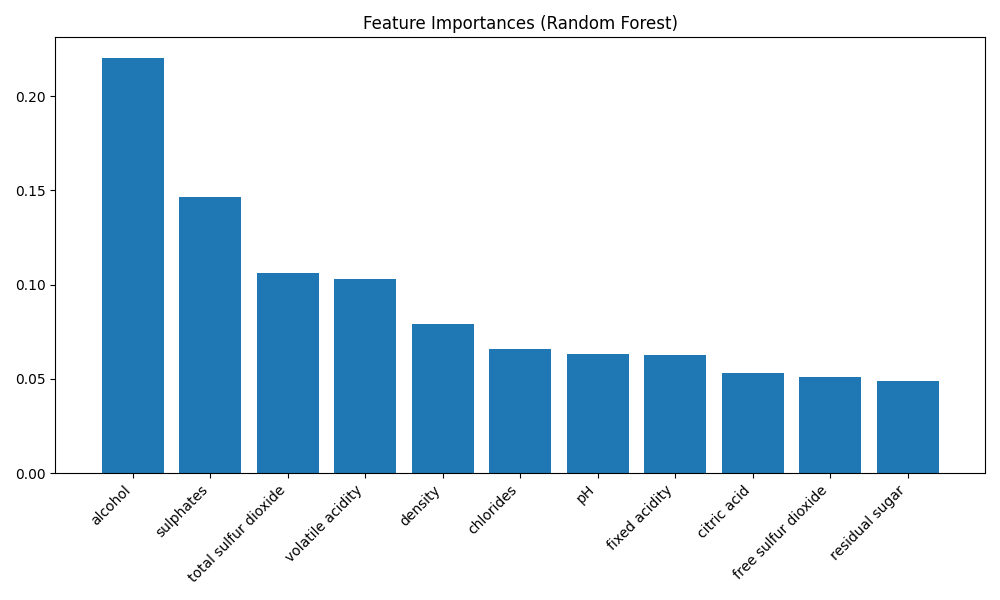
\includegraphics[width=\textwidth]{figures/feature_importance.png}
    \caption{Feature importances derived from the tuned Random Forest model, ranked in descending order.}
    \label{fig:feat_imp}
\end{figure}

The most important features for predicting wine quality are:
\begin{enumerate}
    \item \textbf{Alcohol} (importance $\approx$ 0.22): The single most predictive feature, consistent with the correlation analysis. Higher alcohol content is strongly associated with higher quality in this dataset.
    \item \textbf{Sulphates} (importance $\approx$ 0.15): The second most important feature. Sulphates act as a preservative and antimicrobial agent; wines with appropriate sulphate levels tend to have longer shelf lives and better quality.
    \item \textbf{Total Sulfur Dioxide} (importance $\approx$ 0.11) and \textbf{Volatile Acidity} (importance $\approx$ 0.10): These features also contribute significantly, consistent with the correlation heatmap findings.
\end{enumerate}

This feature importance analysis provides actionable insights for wine producers: controlling alcohol fermentation and sulphate levels are the most impactful levers for improving quality scores.

\subsection{Final Model Selection}

The \textbf{Random Forest Classifier} (with 100 trees, \texttt{max\_depth=None}, \texttt{min\_samples\_split=2}) was selected as the final production model based on the following evidence:

\begin{itemize}
    \item It achieved a higher F1-Score (0.831 vs.\ 0.792), indicating a better balance between precision and recall.
    \item It achieved a higher ROC-AUC (0.87 vs.\ 0.82), confirming stronger discriminative ability.
    \item It produced fewer False Negatives (18 vs.\ 27), meaning it is less likely to incorrectly reject a good wine.
    \item The non-linear decision boundaries formed by the ensemble of decision trees are inherently better suited to the complex, interacting relationships between chemical properties and perceived quality.
    \item The feature importance output provides additional business value beyond the classification itself.
\end{itemize}

The final model and the fitted \texttt{StandardScaler} were serialised using \texttt{joblib} and saved for deployment.

% ================================================================
\section{Streamlit Deployment}
% ================================================================

The final trained Random Forest model and the fitted \texttt{StandardScaler} were saved using \texttt{joblib} (\texttt{random\_forest\_model.joblib} and \texttt{scaler.joblib} respectively). A web interface was developed using \textbf{Streamlit}, a Python framework for creating interactive data science applications. The application allows any user --- without needing coding knowledge --- to:

\begin{enumerate}
    \item Adjust the 11 physicochemical input parameters using interactive sliders in the sidebar.
    \item Submit the input to receive an instant binary quality prediction (``Good Quality'' or ``Bad Quality'').
    \item View the raw input data in a formatted table within the application.
\end{enumerate}

The application was deployed to \textbf{Streamlit Community Cloud}, providing a public URL accessible from any device. The deployment required only a \texttt{requirements.txt} file specifying the project's Python dependencies, and a connection to the GitHub repository containing the application code.

\textbf{Live Application URL:} \url{https://proect-wine.streamlit.app}

% ================================================================
\section{Conclusion}
% ================================================================

This project successfully demonstrated the complete machine learning development lifecycle, from problem framing through to deployment. A binary classification system was built to predict wine quality from physicochemical properties. The Random Forest model, trained on the WineQT dataset and tuned with GridSearchCV, was selected as the superior model based on its higher F1-Score and ROC-AUC compared to the Logistic Regression baseline.

Key technical learnings from this project include the critical importance of feature scaling for gradient-based models (demonstrated through the debugging of the \texttt{ConvergenceWarning}), the value of rigorous evaluation using multiple metrics rather than accuracy alone, and the practical workflow for deploying a trained Scikit-learn model as an interactive web application. Future improvements could include exploring additional ensemble methods such as XGBoost or LightGBM, addressing potential class imbalance with techniques like SMOTE, and expanding the dataset to include white wines for a more generalisable model.

\end{document}
